% !TeX program = xelatex
% Local layout based on the official submission-style document.
\documentclass[UTF8,fontset=windows,zihao=5]{ctexart}
\usepackage[a4paper,left=18.01mm,right=20mm,top=20mm,bottom=20mm]{geometry}
\usepackage{amsmath,amssymb,amsthm,bm,booktabs,tabularx,array,graphicx}
\usepackage{setspace,float,caption,xcolor,tikz}
\usetikzlibrary{arrows.meta,positioning}
\usepackage[numbers,sort&compress,square,super]{natbib}
\usepackage{xurl}
\usepackage[unicode,hidelinks]{hyperref}
\setmainfont{Times New Roman}
\setCJKmainfont{SimSun}[BoldFont=SimHei,ItalicFont=KaiTi]
\setCJKsansfont{SimHei}
\setstretch{1.5}
\setlength{\emergencystretch}{2em}
\setlength{\parindent}{2em}
\setlength{\textfloatsep}{10pt}
\setlength{\intextsep}{10pt}
\setcounter{topnumber}{3}
\renewcommand{\topfraction}{.92}
\renewcommand{\textfraction}{.06}
\renewcommand{\floatpagefraction}{.8}
\captionsetup{font=small,labelsep=quad}
\newcommand{\bicaption}[2]{\caption{#1\\#2}}
\newcommand{\E}{\mathbb E}
\newcommand{\R}{\mathbb R}
\newcommand{\TV}{\operatorname{TV}}
\newcommand{\tr}{\operatorname{tr}}
\newcommand{\Law}{\mathcal L}
\newcommand{\ind}{\mathbf 1}
\newcommand{\norm}[1]{\left\|#1\right\|}
\newtheorem{theorem}{定理}
\newtheorem{lemma}{引理}
\newtheorem{proposition}{命题}
\renewcommand{\proofname}{证明}
\renewcommand{\refname}{参考文献}
\pagestyle{plain}
\ctexset{section={format=\large\heiti},subsection={format=\normalsize\heiti}}
\hypersetup{pdftitle={可信反馈下远程估计的隐蔽攻击损伤界},
 pdfsubject={Stealthy-attack damage bounds under trusted prediction feedback}}
\begin{document}
\begin{center}
{\heiti\zihao{3}可信反馈下远程估计的隐蔽攻击损伤界\par}
\end{center}
% Author-controlled fields intentionally omitted by the user's instruction.
% Required before uploading: Chinese/English authors and order, affiliations,
% corresponding author and email, funding statement, classification code.
% Do not invent these values or a journal DOI/volume/acceptance date.

\noindent\textbf{摘\quad 要：}
针对随机触发远程估计中“可信事件反馈”与“可篡改发送载荷”并存的情形，研究统计隐蔽约束如何限制真实均方估计损伤。精确预测反馈下，下一可信静默事件的归一化概率直接依赖隐藏估计偏差；保留协方差标签后，可将指定记录的总变差预算转化为损伤上界。对全状态含噪观测、可逆状态矩阵和固定有限目标时刻，证明全部有界因果攻击下的最坏损伤与攻击幅值平方、记录总变差预算中的较小量同阶。进一步在标量实际预测量化协议下，证明受限事件与量化遥测记录同律仍可伴随正损伤，且其最坏值具有幅值与量化精度平方的匹配阶数。数值结果说明损伤分解、双预算界及量化见证的含义；量化结论不涉及完整接收日志下的不可检测性。

\smallskip
\noindent\textbf{关键词：}随机事件触发；远程状态估计；统计隐蔽性；可信反馈；量化；估计损伤

\section*{引言}
远程状态估计器通过通信网络接收传感器量测，并据此更新状态预测。随机事件触发可依据量测与预测的偏差减少发送次数；在指数二次触发规则下，静默本身也构成估计信息，并可在适当线性高斯模型中保持条件高斯结构\cite{han2015}。

本文关注一个由协议时序产生的矛盾。传感器先依据可信预测反馈决定是否发送，发送位确定后，攻击者才可修改已发送载荷；接收端因此形成偏差，而这个实际预测又会反馈到传感器并影响下一次可信事件。事件记录可能暴露偏差，但审计者看到的统计差异究竟能限制多少真实损伤，并不能仅由“事件可信”直接回答。

我们聚焦三个问题：在攻击峰值与指定记录的总体总变差（total variation，TV）预算同时受限时，精确预测反馈能否对全部允许因果攻击给出真实均方误差（mean-square error，MSE）上界？两项预算如何共同决定最坏损伤的阶数？当实际预测反馈被量化、审计者只保留指定遥测字段时，精确反馈下的零损伤保证会怎样变化？

现有研究已从随机触发估计的创新分布、攻击调度、条件矩约束、可靠信息源和序贯检测等角度研究隐蔽攻击\cite{bai2017,shang2022,guo2025,song2022,xu2023,wei2026}。相关工作中，Shang等提出的 complete Gaussian crater（CGC）分布、历史相关攻击、指定条件下非线性策略的可行性比较，以及可靠信息下的攻击可观测性均有直接成果。表\ref{tab:related}按模型信息、攻击权限和统计约束对比与本文最接近的结果。不同工作的攻击者信息与隐蔽准则不相同；条件矩约束、检测器通过条件和联合记录TV预算不是可互换的指标。

\begin{table}[ht]
\centering\scriptsize
\bicaption{与相关工作的定理级问题对照}{Table \thetable\quad Theorem-level comparison with related work}
\label{tab:related}
\begin{tabularx}{\linewidth}{>{\raggedright\arraybackslash}p{1.55cm}*{4}{>{\raggedright\arraybackslash}X}}
\toprule
工作 & 触发与可信信息 & 攻击及隐蔽约束 & 主要性能结论 & 与本文问题的区别\\
\midrule
Shang等\cite{shang2022} & 源端本地随机事件触发 & 创新/通信通道修改；CGC分布与指定攻击条件 & Theorem 2给协方差递推；Theorem 3及Corollary 3给隐蔽攻击构造 & 受攻远端预测不是触发中心\\
Guo等\cite{guo2025} & 源端创新与攻击调度 & 给定信息下的策略；攻击分支条件均值/协方差约束 & Theorem 1比较给定历史和调度下的条件损伤可行策略，包括非线性策略 & 本文约束指定总体记录分布\\
Wei等\cite{wei2026} & 可靠/可疑信息与序贯检测 & 信息源访问受限；时间及交叉矩条件 & Theorem 2给可行集最坏误差；Corollary 1给特定秩条件 & 触发反馈路径和记录预算不同\\
Li等\cite{li2026} & 前向量化创新及反馈辅助信息 & 量化前创新篡改；指定检测器约束 & Theorem 3优化指定符号攻击；Theorem 4给协方差收敛条件 & 本文量化实际预测反馈中心\\
本文 & 可信发送事件及接收端实际预测反馈 & 发送决定后逐路径有界载荷修改；指定记录TV约束 & 有限时域全策略损伤阶数；量化遥测同律下的残余损伤阶数 & 结论限于本文的协议及记录\\
\bottomrule
\end{tabularx}
\end{table}

本文的区别不在于首次发现可信信息可以约束攻击。与允许攻击者在发送决策前替换预测、或向传感器广播健康预测的模型\cite{song2022,xu2023,wei2026}不同，我们要求反馈忠实于接收端实际预测，事件位不可伪造，载荷修改发生在真实发送决定之后。因而隐藏估计偏差进入下一可信事件的条件概率。结合目标时刻的协方差标签，可校准不同事件历史的健康静默基准。

其关键统计关系将在第\ref{sec:exact}节建立：给定扩充分析历史，下一静默事件的归一化概率等于隐藏偏差的指数二次函数。状态矩阵可逆时，该函数对每个非零偏差严格小于健康值。协方差标签用于控制事件历史概率变化对真实MSE分解中协方差项的影响。由此，峰值限制控制偏差范围，TV预算控制记录可见的总体统计变化，两者共同给出全策略损伤界；构造性下界证明该阶数不能统一改进。

量化反馈扩展用于说明这一保证的适用边界。前向量化观测篡改、量化通信调度以及量化创新下的事件触发估计已有研究\cite{li2026,li2025,shen2025}；本文改变的是进入触发规则的实际预测中心，并明确区分接收端内部信息与审计者记录。量化中心进入触发规则后，多个内部预测可映射为同一反馈码。攻击者可在码格内改变估计而不改变指定的事件及量化遥测记录，因此零TV时仍可能存在正损伤。该结论只针对标量、无饱和量化协议和明确给定的受限记录，不推出完整接收日志下的不可检测性。

本文的理论贡献是上述两个协议下的有限时域损伤界，不是新的触发器、估计器或检测算法。数值部分用于解释真实损伤分解、双预算上下界与量化见证；有限样本不能替代总体定理。本文未证明特定工业系统满足全部信任条件，也未证明受限遥测比完整载荷认证成本更低。全文安排如下：第1节定义系统、攻击权限和记录；第2节给出精确反馈下的损伤机制与定理；第3节分析量化反馈下的残余损伤；第4节报告数值结果；第5节总结适用范围。

\section{系统、信息与损伤模型}
\subsection{精确反馈协议}
考虑固定有限维线性高斯模型
\begin{equation}
{\bm{x}}_{t+1}={\bm{A}}{\bm{x}}_t+{\bm{w}}_t,\qquad {\bm{y}}_t={\bm{x}}_t+{\bm{v}}_t .
\label{eq:model}
\end{equation}
设 ${\bm{x}}_0\sim N({\bm{m}}_0,{\bm{P}}_0)$，${\bm{w}}_t\sim N(0,{\bm{Q}})$，${\bm{v}}_t\sim N(0,{\bm{R}})$，
${\bm{P}}_0,{\bm{R}},{\bm{Z}}\succ0$，${\bm{Q}}\succeq0$，${\bm{A}}$可逆；初态、全部过程噪声、量测噪声和触发随机数相互独立。
物理系统不受估计输出控制，不包含自然丢包、时延或乱序。
传感器取得可信实际预测${\bm{m}}_t^-$后，使用私有独立$U_t\sim\mathrm{Unif}[0,1]$决定
\begin{equation}
\gamma_t=0\quad\Longleftrightarrow\quad
U_t\le g({\bm{y}}_t-{\bm{m}}_t^-),\qquad g({\bm{z}})=e^{-{\bm{z}}^\top {\bm{Z}}{\bm{z}}/2}.
\label{eq:trigger}
\end{equation}
发送位已确定后，载荷变为$\tilde {\bm{y}}_t={\bm{y}}_t+{\bm{a}}_t$，
$\norm{{\bm{a}}_t}\le b$；静默时${\bm{a}}_t=0$。

令 ${\bm{R}}_1={\bm{R}},\ {\bm{R}}_0={\bm{R}}+{\bm{Z}}^{-1}$，
${\bm{K}}_i({\bm{P}})={\bm{P}}({\bm{P}}+{\bm{R}}_i)^{-1}$，$F_i({\bm{P}})={\bm{P}}-{\bm{P}}({\bm{P}}+{\bm{R}}_i)^{-1}{\bm{P}}$。
接收器按既定名义规则更新
\begin{align}
{\bm{m}}_t^+&={\bm{m}}_t^-+\gamma_t{\bm{K}}_1({\bm{P}}_t^-)(\tilde {\bm{y}}_t-{\bm{m}}_t^-),&
{\bm{P}}_t^+&=F_{\gamma_t}({\bm{P}}_t^-),\label{eq:receive}\\
{\bm{m}}_{t+1}^-&={\bm{A}}{\bm{m}}_t^+,& {\bm{P}}_{t+1}^-&={\bm{A}}{\bm{P}}_t^+{\bm{A}}^\top+{\bm{Q}}.\nonumber
\end{align}
初值为$({\bm{m}}_0,{\bm{P}}_0)$。${\bm{P}}_t^\pm$是由事件历史确定的名义协方差标签；
在受攻时，它不能单独代表实际接收估计器的真实MSE。

\subsection{信息域与合法策略}
用$\omega_a$表示独立于物理过程和触发随机数的修改方私有种子，
$Y_t^{\rm true}={\bm{y}}_t$在发送时成立，否则为$\bot$。
定义扩充分析信息
\[
\mathcal G_t^-=\sigma(\omega_a,\gamma_{0:t-1},Y^{\rm true}_{0:t-1}),\qquad
\mathcal G_t^+=\mathcal G_t^-\vee\sigma(\gamma_t,Y_t^{\rm true}).
\]
允许任意$\mathcal G_t^+$可测且满足峰值的随机因果策略。
策略不能读取真实状态、未发送量测、未来噪声或$U_t$。
给定策略，已实施动作和接收预测可由上述历史重建。
扩充信息用于证明条件分布，不授予审计者真实量测副本。

固定目标$k$，损伤为同一协议内部的真实MSE增量
\begin{equation}
J_k(\pi)=\E_\pi\norm{{\bm{x}}_k-{\bm{m}}_k^+}^2-\E_0\norm{{\bm{x}}_k-{\bm{m}}_k^+}^2.
\label{eq:damage}
\end{equation}
单个策略的增量可为负；零策略可行，最坏值非负。
定义记录字段
\[
\tilde {\bm{y}}_t^{\rm rec}=\begin{cases}
\tilde {\bm{y}}_t,&\gamma_t=1,\\
\bot,&\gamma_t=0.
\end{cases}
\]
截至$k+1$的完整日志为
\[
H_{k+1}=\bigl(\gamma_{0:k+1},\ m^-_{0:k+1},\ \tilde y^{\rm rec}_{0:k+1}\bigr).
\]
其中事件位和实际预测反馈均可信；载荷字段记录接收端实际收到的值，但不表示该值具有源端完整性认证。
静默以$\bot$编码，因而不会与丢包混淆。
考虑记录
\[
R_{\rm full}=H_{k+1},\qquad
R_{\rm bits}=\gamma_{0:k+1},\qquad
R_m=({\bm{P}}_k^+,\gamma_{k+1}).
\]
定义
\begin{equation}
\Delta_R(\pi)=\TV(\Law_\pi(R),\Law_0(R)),\qquad
V_R^{(k)}(b,\varepsilon)=
\sup_{\pi:\,\norm{{\bm{a}}_t}\le b,\,\Delta_R(\pi)\le\varepsilon}J_k(\pi).
\label{eq:value}
\end{equation}
本文取$\TV(\mu,\nu)=\sup_B|\mu(B)-\nu(B)|$，向量范数为欧氏范数，矩阵范数为其诱导谱范数。
TV约束为总体分布条件，既非一次运行的观测值，也非预设误报率。
任意仅使用该记录的检验，其攻击与健康拒绝概率之差不超过$\Delta_R$；
这一标准性质解释了统计隐蔽预算的含义。

\begin{figure}[ht]
\centering
\begin{tikzpicture}[
  block/.style={draw,align=center,text width=36mm,minimum height=13mm,font=\small},
  signal/.style={-{Latex[length=1.8mm]},semithick},
  audit/.style={-{Latex[length=1.6mm]},densely dashed}
]
\node[block] (sensor) {传感器获得可信预测并决定事件};
\node[block,right=18mm of sensor] (attacker) {发送决定后修改发送载荷};
\node[block,right=18mm of attacker] (receiver) {接收端更新估计并产生实际预测};
\node[block,below=17mm of attacker,text width=145mm,minimum height=9mm] (auditor)
  {完整日志记录事件位、可信预测反馈及接收载荷；载荷只表示接收值，不表示源端认证};
\draw[signal] (sensor.east) -- node[midway,above=2mm,fill=white,inner sep=1pt,font=\footnotesize]{仅发送时} (attacker.west);
\draw[signal] (attacker.east) -- node[midway,above=2mm,fill=white,inner sep=1pt,font=\footnotesize]{修改后载荷} (receiver.west);
\draw[signal] (receiver.north) .. controls +(0,13mm) and +(0,13mm) ..
  node[above,font=\small]{下一时刻实际预测反馈} (sensor.north);
\draw[audit] (sensor.south) -- (auditor.north west);
\draw[audit] (attacker.south) -- (auditor.north);
\draw[audit] (receiver.south) -- (auditor.north east);
\end{tikzpicture}
\bicaption{发送决定、载荷修改和可信审计字段的时序}{Fig. \thefigure\quad Timing of transmission, payload modification, and trusted audit fields}
\label{fig:protocol}
\end{figure}

图\ref{fig:protocol}中的完整日志比主定理使用的每种记录都更丰富。
特别是$R_m$仅保留目标协方差标签及下一事件，$R_{\rm bits}$只保留事件串；
量化扩展另行定义量化遥测记录，不把载荷字段默认为可信。

\subsection{评价者与记录可信性}
远端估计器拥有连续载荷及内部预测，外部审计者可只订阅已规定的可信事件和控制反馈。
载荷未经完整性保护不妨碍保存收到的值；是否向审计者提供它由所规定的信息接口决定。
本文量化扩展把审计者限制为控制遥测订阅者，增强审计则明确加入额外字段。
静默与缺包必须区分，反馈码必须对应传感器实际采用的值，模型版本及初始化已知。
若这些条件不成立，不能直接应用下面的保证。

\section{精确反馈下的损伤保证}
\label{sec:exact}
\subsection{损伤分解与下一事件统计机制}
给定$\mathcal G_t^\pm$，真实状态仍具有高斯条件分布，条件均值记${\bm{\mu}}_t^\pm$，
协方差为${\bm{P}}_t^\pm$。发送并给定真实测量后，事件似然因子在后验归一化时消去；
静默时，积分量测噪声得到以实际预测为中心的高斯似然。该结构不要求载荷修改与当前量测独立。
令${\bm{d}}_t={\bm{\mu}}_t^--{\bm{m}}_t^-$、${\bm{D}}_t={\bm{\mu}}_t^+-{\bm{m}}_t^+$，则
\begin{align}
{\bm{D}}_t&=({\bm{I}}-{\bm{K}}_{\gamma_t}({\bm{P}}_t^-)){\bm{d}}_t-\gamma_t{\bm{K}}_1({\bm{P}}_t^-){\bm{a}}_t,\qquad
{\bm{d}}_{t+1}={\bm{A}}{\bm{D}}_t,\label{eq:bias}\\
J_k&=\E_\pi\norm{{\bm{D}}_k}^2+
\E_\pi\tr {\bm{P}}_k^+-\E_0\tr {\bm{P}}_k^+.\label{eq:split}
\end{align}
式\eqref{eq:split}由条件零均值残差的正交性得到。最后两项不能删除；
事件概率改变可能使其为负。

固定${\bm{P}}={\bm{P}}_k^+$，记下一静默位$Y=\ind_{\{\gamma_{k+1}=0\}}$，定义
\begin{align}
{\bm{\Sigma}}({\bm{P}})&={\bm{A}}{\bm{P}}{\bm{A}}^\top+{\bm{Q}}+{\bm{R}},\qquad
s({\bm{P}})=\det({\bm{I}}+{\bm{Z}}^{1/2}{\bm{\Sigma}}({\bm{P}}){\bm{Z}}^{1/2})^{-1/2},\nonumber\\
{\bm{H}}({\bm{P}})&=\tfrac12 {\bm{A}}^\top[{\bm{Z}}^{-1}+{\bm{\Sigma}}({\bm{P}})]^{-1}{\bm{A}},\qquad
W=Y/s({\bm{P}}).
\end{align}
真实条件创新的均值为${\bm{A}}{\bm{D}}_k$。高斯积分给
\begin{equation}
\E_\pi[Y\mid\mathcal G_k^+]=s({\bm{P}})e^{-{\bm{D}}_k^\top {\bm{H}}({\bm{P}}){\bm{D}}_k},
\qquad \E_0W=1,\quad \E_\pi W=\E_\pi e^{-{\bm{D}}_k^\top {\bm{H}}({\bm{P}}){\bm{D}}_k}.
\label{eq:witness}
\end{equation}
未来载荷修改发生在未来事件之后，故不改变这一关系。

式\eqref{eq:witness}是可信事件转化为损伤信息的关键。给定历史时，下一静默概率相对健康基准$s({\bm{P}})$乘以$\exp[-{\bm{D}}_k^\top {\bm{H}}({\bm{P}}){\bm{D}}_k]$；由于${\bm{A}}$可逆且${\bm{Z}}^{-1}+{\bm{\Sigma}}({\bm{P}})\succ0$，有${\bm{H}}({\bm{P}})\succ0$，每个非零偏差都会严格降低该归一化概率。审计者无需直接观察${\bm{D}}_k$，而是比较记录中${\bm{P}}_k^+$与下一事件的联合分布。

协方差标签的作用是校准事件历史对应的基准概率$s({\bm{P}})$。若只比较未校准的静默边缘概率，攻击改变不同事件历史的权重也会改变平均静默率，不能将其全部归因于隐藏偏差。式\eqref{eq:split}中的协方差分布变化项同样必须保留；定理对$R_{\rm bits}$和$R_{\rm full}$成立，是因为这些记录也保留了${\bm{P}}_k^+$所依赖的事件历史，而不是因为这些字段具有相同的信息量。

有限$k$下，P及增益取有限值。由式\eqref{eq:bias}可得
$\norm{{\bm{D}}_k}\le r_kb$。固定$b_{\rm ref}>0$，取
\[
h_*=\min_{\bm{P}}\lambda_{\min}({\bm{H}}({\bm{P}}))>0,\quad
B_*=r_kb_{\rm ref},\quad q=\frac{1-e^{-h_*B_*^2}}{B_*^2}>0.
\]
其中${\bm{A}}$可逆保证$h_*>0$。割线不等式给出
\begin{proposition}[可信下一事件给出的总体损伤上界]
对全部允许策略及$0\le b\le b_{\rm ref}$，
\begin{equation}
J_k\le \frac{1-\E_\pi W}{q}
+\E_\pi\tr {\bm{P}}_k^+-\E_0\tr {\bm{P}}_k^+.
\label{eq:certificate}
\end{equation}
\end{proposition}
\begin{proof}
在$\norm{{\bm{D}}_k}\le B_*$上，
$1-e^{-{\bm{D}}_k^\top {\bm{H}}({\bm{P}}){\bm{D}}_k}\ge q\norm{{\bm{D}}_k}^2$。
对式\eqref{eq:witness}取期望并代入式\eqref{eq:split}即得。
\end{proof}
右侧是由可信事件与已知模型标签定义的总体统计量，不需要审计者知道攻击向量或真实状态。
有限样本估计仍有统计余量；一个事件或一条轨迹不能直接认证总体损伤。

\subsection{双预算阶数及完整日志下界}
记$\Delta_m=\Delta_{R_m}$，
令$M=\max_{\bm{P}}1/s({\bm{P}})$，$\Omega_k=\max_{\bm{P}}\tr {\bm{P}}-\min_{\bm{P}}\tr {\bm{P}}$。
因$0\le W\le M$且${\bm{P}}$在记录中，标准TV期望界给
\[
J_k\le(M/q+\Omega_k)\Delta_m.
\]
另一方面，式\eqref{eq:bias}控制偏差平方；每个历史下静默概率相对健康变化为$O(b^2)$。
对有限事件前缀耦合并控制P标签的期望差，得到$J_k\le C_{\rm peak}b^2$。
该第二步不可仅从偏差半径推出而忽略协方差项。

\begin{theorem}[精确反馈的有限时域损伤阶数]
\label{thm:exact}
固定模型、有限维数、目标$k$及$b_{\rm ref}$，存在正有限常数$c,C$，
对$0<b\le b_{\rm ref}$、$0\le\varepsilon\le1$及
$R\in\{R_{\rm full},R_{\rm bits},R_m\}$，
\begin{equation}
c\min\{b^2,\varepsilon\}\le V_R^{(k)}(b,\varepsilon)
\le C\min\{b^2,\varepsilon\}.
\label{eq:exact-bound}
\end{equation}
特别地，$V_R^{(k)}(b,0)=0$。
\end{theorem}
\begin{proof}
上界为两种界的组合及记录的数据处理。
下界在目标前不修改，仅在目标真实发送后使用独立等概率符号$\sigma$和固定单位方向${\bm{v}}$，$\norm {\bm{v}}=1$，
取${\bm{a}}_k=\sigma\eta {\bm{v}}$，其他时刻为零。目标损伤为$L_{\bm{v}}\eta^2$，$L_{\bm{v}}>0$。
给定健康前史，将当前连续载荷和下一静默原子/连续载荷写成一个联合核。
该核对位移二阶连续$L^1$可微，正负混合的一阶项消去，完整日志TV不超过$C_1\eta^2$。
取$\eta=\min\{b,\sqrt{\varepsilon/C_1}\}$完成下界，联合核细节见附录\ref{app:single}。
\end{proof}
单拍构造足够支持阶数，并不声称是精确最坏策略。
常数依赖模型、$k$、$b_{\rm ref}$；$\varepsilon$与$b^2$的量纲通过模型相关常数联系，
两预算切换点不是普遍的$\varepsilon=b^2$。
三个记录的最坏损伤具有相同阶数，不表示它们的最坏值或上界常数相等。
由于$R_m$、$R_{\rm bits}$均为$R_{\rm full}$的确定性投影，数据处理给出
$V_{R_{\rm full}}^{(k)}\le V_{R_{\rm bits}}^{(k)}\le V_{R_m}^{(k)}$；
定理说明的是这三个量在固定模型和时域下具有匹配阶数。

\subsection{观察时域与信息限制}
式\eqref{eq:witness}使用下一拍可信事件以及目标协方差标签。
因此，定理\ref{thm:exact}不直接适用于只观察到目标拍的日志，或删去历史校准标签后的单个事件边缘。
这一充分保证不声称已确定所有审计方式的最小记录。
精确协方差标签由事件历史决定，但并不天然构成低比特压缩；
本文未给出其固定字长编码或通信成本最优性。

\section{有限反馈精度下的保证退化}
精确反馈定理依赖传感器使用接收端实际预测形成事件。现在改变协议本身：传感器改用量化预测中心触发，接收端也围绕该中心执行一致的静默更新。这样，内部预测在同一量化格内移动时，反馈码及事件记录可以保持不变；下文刻画由此产生的残余损伤，并区分协议量化与仅删减审计字段这两种变化。

\subsection{量化协议及一致静默更新}
本节限于\textbf{标量}系统，$A\ne0$，$P_0,R,Z>0$，$Q\ge0$，并固定有限目标$k$。
量化的是实际预测反馈，前向发送载荷保持连续。取无限格点、无饱和的均匀量化器
\[
c_t=Q_\delta(m_t^-),\qquad Q_\delta(m)=2\delta\left\lfloor\frac{m+\delta}{2\delta}\right\rfloor,
\qquad |c_t-m_t^-|\le\delta,
\]
量化格为半开区间$[2j\delta-\delta,2j\delta+\delta)$，$j\in\mathbb Z$，故并列点归属固定。
传感器用$y_t-c_t$生成原指数二次随机事件。
发送支路保持原更新；静默时必须使用
\begin{equation}
m_t^+=m_t^-+K_0(P_t^-)(c_t-m_t^-),\qquad P_t^+=F_0(P_t^-).
\label{eq:silentq}
\end{equation}
健康条件均值于是与接收均值一致。若仍使用旧的$m_t^+=m_t^-$，
健康运行也会因非零舍入误差产生条件均值失配。

给定扩充真实历史，$c_t$为已知量；静默似然是以$c_t$为中心、噪声$R+Z^{-1}$的高斯因子。
发送并给定真实测量后事件因子仍可消去。因此精确条件高斯结构保留，
且真实条件均值与接收均值的偏差仍满足式\eqref{eq:bias}。
量化误差项在两者使用同一静默中心后相消。
这个结论不应移到只包含量化码或污染载荷的较小条件信息域。

定义同量化协议内部损伤
\[
J_{k,\delta}=\E_{\pi,\delta}(x_k-m_k^+)^2-\E_{0,\delta}(x_k-m_k^+)^2.
\]
它不含正常量化运行相对正常精确运行的损失。
令$T_{\delta,k}=(\gamma_{0:k+1},c_{0:k+1},P_k^+)$为全部可信控制遥测，
$R_{m,\delta}=(P_k^+,c_{k+1},\gamma_{k+1})$为其投影。
两者都排除连续接收载荷和未量化内部预测。
相应TV与最坏值采用式\eqref{eq:value}的同协议定义。

\subsection{零记录差异下的残余损伤}
令$e=c_{k+1}-m_{k+1}^-$，$P=P_k^+$，
$\Sigma(P)=A^2P+Q+R$，$V(P)=Z^{-1}+\Sigma(P)$，$h(P)=A^2/[2V(P)]$。
下一事件关系变为
\begin{equation}
\E_{\pi,\delta}[W\mid\mathcal G_k^+]
=\exp[-h(P)(D_k-e/A)^2],\qquad W=Y/s(P).
\label{eq:qprob}
\end{equation}
健康时$D_k=0$，所以$\E_{0,\delta}W$一般小于1；
原精确协议的健康归一化不能直接沿用。

\begin{theorem}[标量有限精度下的零TV残余损伤阶数]
\label{thm:quant}
固定标量模型、有限$k$、$b_{\rm ref}>0$、$\delta_{\rm ref}>0$。
存在$\delta_*>0$及正有限$c_k,C_k$，使全部
$0<b\le b_{\rm ref}$、$0<\delta\le\min\{\delta_*,\delta_{\rm ref}\}$满足
\begin{equation}
c_k\min\{b^2,\delta^2\}\le V_{R,\delta}^{(k)}(b,0)
\le C_k\min\{b^2,\delta^2\},
\label{eq:quant-bound}
\end{equation}
其中$R=T_{\delta,k}$或$R_{m,\delta}$。
\end{theorem}
\begin{proof}
上界适用于包括目标前动作在内的全部允许策略。
有限前缀集给$|D_k|\le r_kb$。取
$R_*=r_kb_{\rm ref}+\delta_{\rm ref}/|A|$，
$h_*=\min_Ph(P)>0$，
$q_*=(1-e^{-h_*R_*^2})/R_*^2$，
$c_0=\max_P1/[2V(P)]$。
当记录同律，$\E_\pi W=\E_0W$且P标签同律。
由式\eqref{eq:qprob}和健康量化误差界，
\[
q_*\E_\pi(D_k-e/A)^2\le1-\E_\pi W
=1-\E_0W\le c_0\delta^2.
\]
于是
\[
J_{k,\delta}=\E_\pi D_k^2
\le\left(\sqrt{c_0/q_*}+|A|^{-1}\right)^2\delta^2,
\qquad J_{k,\delta}\le r_k^2b^2 .
\]

下界选择此前无动作的合法子类。给定健康真实前史$\zeta$，
令$m=m_k^-$、$e_k=c_k-m$、$P_h=P_k^-$、$S_h=P_h+R$、$K_h=P_h/S_h$。
当前创新$u=y_k-m$的发送次密度为
\begin{equation}
f_{h,e_k}(u)=\phi_{S_h}(u)[1-\exp(-Z(u-e_k)^2/2)].
\label{eq:sentq}
\end{equation}
真实发送后，下一健康预测$M=A(m+K_hu)$可由合法信息计算。
定义开中央半区
\[
\mathcal C_\delta=\bigcup_{j\in\mathbb Z}
(2j\delta-\delta/2,\,2j\delta+\delta/2).
\]
只在真实发送且$M\in\mathcal C_\delta$时，选择独立符号动作$\sigma\eta$，
$\eta=\min\{b,\delta/(2\alpha_{\max})\}$，
$\alpha_{\max}=\max_h|AK_h|$。
因$|AK_h|\eta\le\delta/2$且中央区为开集，两种符号均严格不跨格，下一实际反馈码及事件逐路径相同，
目标前的全部事件/反馈也相同。
独立符号消去目标误差交叉项，故
\[
J_{k,\delta}=\eta^2\E_{0,\delta}[K_h^2\ind_E].
\]
附录\ref{app:uniform}证明安全发送事件的概率在所有健康前史下至少$p_*/4>0$，
从而给出式\eqref{eq:quant-bound}的正下界。
\end{proof}

定理\ref{thm:quant}与定理\ref{thm:exact}形成一组适用范围对照：精确反馈下，指定记录TV为零强制最坏损伤为零；量化反馈下，受限遥测同律仍允许$\Theta(\min\{b^2,\delta^2\})$的残余损伤。这里失效的是量化协议及其指定审计记录下的严格零损伤保证，不是对完整接收日志的不可检测性结论。

定理\ref{thm:quant}的常数可依赖$k$，不是长时间一致界。
其下界取目标前无动作策略，只是全允许策略类的合法子集；
不需要也没有假设所有允许攻击此前均无动作。
$\delta^2$在该记录下是不能统一缩为$o(\delta^2)$的余量，
不表示每条运行均有损伤。

\subsection{协议变化与信息变化的区别}
\begin{table}[ht]\centering\small
\bicaption{反馈协议与审计记录的区别}{Table \thetable\quad Feedback protocols and audit records}
\begin{tabularx}{\linewidth}{lXX}
\toprule
Setting & Actual trigger center & Proven guarantee\\
\midrule
A: exact feedback & $m_t^-$ & Zero record TV implies zero worst-case damage.\\
B: quantized feedback & $Q_\delta(m_t^-)$ & Identical telemetry laws allow the residual damage in \eqref{eq:quant-bound}.\\
C: enhanced audit & Same as B & Additional payload or exact prediction information cannot increase worst-case damage; a general zero-damage guarantee is unknown.\\
\bottomrule
\end{tabularx}
\end{table}
仅把A的日志显示值量化，同时传感器仍使用精确中心，不会破坏原先由P和下一事件给出的保证。
B的地板来自量化中心进入实际触发，以及审计者不保留足以区分该见证的连续数据共同作用。

对于定理下界中的独立符号见证，加入目标拍收到的连续载荷后，
统计量$\gamma_k\tilde y_k^2$的期望差为$\eta^2\Pr(E)>0$；
加入下一未量化预测后，其平方期望差为$A^2\eta^2\E[K_h^2\ind_E]>0$。
有限二阶矩下，这些差异证明该见证不再同律。
但排除这个见证不等于排除全部零TV策略；对C只可一般地使用记录投影给出$V_C\le V_B$。

无饱和均匀格代表绝对精度假设，其整数索引没有全路径固定字长。
本文不据此给固定比特部署或认证成本优势，也不将采样估计TV替代上述严格同律证明。

\section{数值结果与机制讨论}
本节用已有二维计算和预先规定的标量样本解释定理所表达的量，不以有限样本代替总体结论，也不把一条构造攻击当成最坏策略。结果均来自仓库中已保存的数据；本轮没有重新运行仿真或生成随机样本。

\subsection{精确反馈下的真实损伤与双预算界}
二维算例采用
\[
{\bm{A}}_{\rm S}=\begin{bmatrix}.82&.18\\-.10&.72\end{bmatrix},\qquad
{\bm{A}}_{\rm U}=\begin{bmatrix}1.04&.12\\.03&.91\end{bmatrix},
\]
\[
{\bm{P}}_0=\begin{bmatrix}.8&.12\\.12&.6\end{bmatrix},\quad
{\bm{Q}}=\begin{bmatrix}.05&.01\\.01&.04\end{bmatrix},\quad
{\bm{R}}=\begin{bmatrix}.2&.03\\.03&.3\end{bmatrix},\quad
{\bm{Z}}=\begin{bmatrix}2&.25\\.25&1.5\end{bmatrix}.
\]
目标时刻为$k=4$，攻击幅值上限为$b=0.1$。表\ref{tab:damage-decomp}比较持续定向策略与目标拍随机符号、下一拍补偿的合法策略。

\begin{table}[ht]
\centering\footnotesize
\bicaption{真实目标损伤的偏差与协方差分解}{Table \thetable\quad Bias and covariance decomposition of true target damage}
\label{tab:damage-decomp}
\begin{tabular}{llrrr}
\toprule
模型 & 策略 & 偏差能量 & 协方差变化 & 真实损伤$J$\\
\midrule
S & 持续定向 & .001315759 & -.000020445 & .001295314\\
U & 持续定向 & .003252364 & -.000120021 & .003132343\\
S & 两拍符号补偿 & .000321850 & $\simeq0$ & .000321850\\
U & 两拍符号补偿 & .000573797 & $\simeq0$ & .000573797\\
\bottomrule
\end{tabular}
\end{table}

持续策略的协方差变化为负，说明真实MSE增量不等于条件偏差能量；忽略事件历史概率变化会高估这两个例子的损伤。两拍策略在目标前无动作，故目标协方差分布不变。其总体统计上界分别为$0.000457526$和$0.000902386$，对应真实损伤的$1.42$倍和$1.57$倍。事件树结果曾在$b=0.2$下由每组40万次独立重置模拟交叉检查；该检查只核对数值实现，不是定理的依据。

图\ref{fig:budget}展示同一模型在$k=4,b=0.1$下随完整日志TV预算变化的解析界。下界由合法构造给出，上界适用于全部允许攻击；图中不是对$V_{R_{\rm full}}^{(k)}$的数值优化或置信区间。两条界之间的间距反映当前证书的保守程度，不应解释为实际最坏值。

\begin{figure}[ht]
\centering
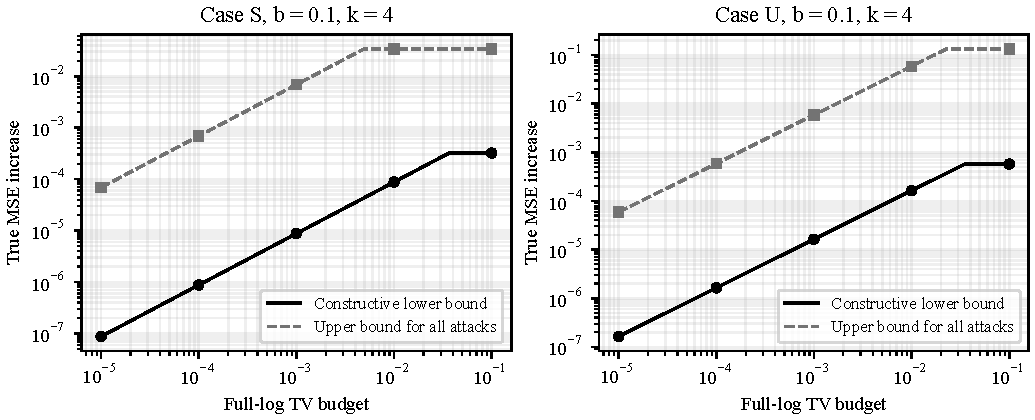
\includegraphics[width=.96\linewidth]{figures/vector_budget.pdf}
\bicaption{固定幅值下的完整日志双预算损伤界（$k=4,b=0.1$）}{Fig. \thefigure\quad Full-log damage bounds under a fixed peak budget ($k=4,b=0.1$)}
\label{fig:budget}
\end{figure}

\subsection{量化反馈下的残余损伤}
标量验证取$A=0.82$（S1）和$A=1.04$（U1），$P_0=0.8$、$Q=0.05$、$R=0.2$、$Z=2$，$k=4$、$b=0.1$。每个模型使用预先固定的2048个独立基础样本，三个量化精度共用配对样本。表\ref{tab:e1-damage}和图\ref{fig:e1}报告B协议中所构造攻击的损伤；它们不是最坏值$V_{R,\delta}^{(k)}$的数值求解。区间为按基础样本配对的探索性bootstrap区间，不是全策略置信界。

\begin{table}[ht]
\centering\footnotesize
\bicaption{B协议中量化见证的目标损伤}{Table \thetable\quad Target damage of the quantized-feedback witness under protocol B}
\label{tab:e1-damage}
\begin{tabular}{lrrrr}
\toprule
模型/精度 & $\delta$ & $10^6\hat J$ & 探索性95\%区间（$10^{-6}$） & $\hat J/\delta^2$\\
\midrule
S1/1 & .00290706 & .295503 & [.256237,.334963] & .034967\\
S1/2 & .00581412 & 1.239223 & [1.086202,1.391006] & .036659\\
S1/3 & .01162823 & 4.814492 & [4.227691,5.429128] & .035606\\
U1/1 & .00556494 & .785686 & [.703663,.878413] & .025370\\
U1/2 & .01112988 & 2.793531 & [2.458229,3.128096] & .022551\\
U1/3 & .02225976 & 11.211802 & [9.942383,12.533812] & .022627\\
\bottomrule
\end{tabular}
\end{table}

本设计令攻击幅值随$\delta$变化且远小于$b$，只覆盖精度主导区。它没有数值检验定理中幅值主导区，也不据三个精度点估计渐近指数。在最大预设精度下，见证损伤约为相应健康MSE的$0.0051\%$（S1）和$0.0077\%$（U1）。这支持“指定遥测下严格零TV保证失效且残余损伤为正”的数学结论，不支持显著工程损害或量化带来正常精度/通信收益的说法。

\begin{figure}[ht]
\centering
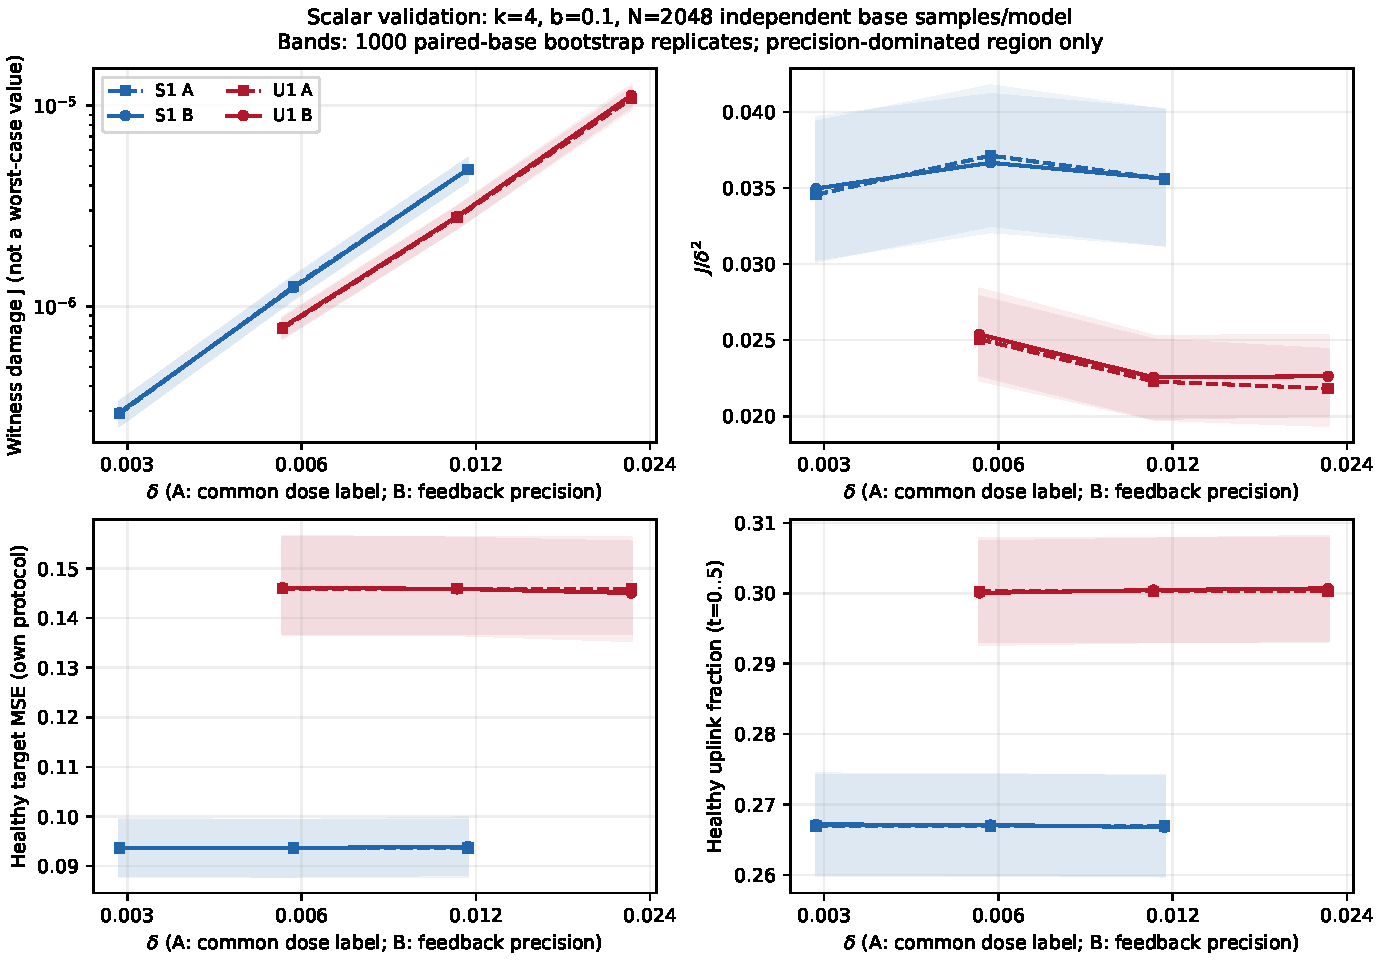
\includegraphics[width=\linewidth]{figures/e1_mechanism.pdf}
\bicaption{量化见证损伤、精度尺度及健康代价}{Fig. \thefigure\quad Quantized-witness damage, precision scaling, and healthy cost}
\label{fig:e1}
\end{figure}

\subsection{记录分辨率与增强审计}
本批A协议每组2048个基础样本均未出现健康与受攻事件串分叉。因此样本事件差为零只反映本次有限样本的分辨率，不能作为总体TV为零的证据；定理中的总体差异由条件概率恒等式支持。相应条件得分差很小，且该诊断使用模拟中的完整条件历史与策略变量，不能解释为审计者已从有限日志中识别出差异。

增强审计C把同一B运行中的连续载荷或未量化预测加入记录。表\ref{tab:e1-c}只列最大预设精度下的代表值：它们与理论矩差一致，足以区分本文构造的独立符号见证，但不证明C能排除所有零TV正损伤策略。对任意攻击，增加字段只给出$V_C\le V_B$。

\begin{table}[ht]
\centering\footnotesize
\bicaption{最大预设精度下增强审计C的代表性矩差}{Table \thetable\quad Representative moment gaps under enhanced audit C at the largest tested precision}
\label{tab:e1-c}
\begin{tabular}{lrr}
\toprule
模型 & 载荷平方差（$10^{-6}$） & 预测平方差（$10^{-6}$）\\
\midrule
S1/3 & 34.445971 & 3.237265\\
U1/3 & 41.684819 & 12.126685\\
\bottomrule
\end{tabular}
\end{table}

综上，二维结果解释了偏差项和协方差项为何必须共同进入真实损伤；预算曲线区分了可达下界与全策略上界；标量结果则说明量化反馈及受限审计记录下的严格隐蔽边界。数值结果没有独立证明一般时域或全部因果策略的结论。

\section{结论}
本文研究了随机触发远程估计中可信预测反馈与可篡改载荷并存时，指定记录能够为真实估计损伤提供何种约束。精确反馈使隐藏估计偏差进入下一可信事件的条件概率；目标协方差标签校准不同事件历史的健康基准。基于这两点，本文对全部允许的有界因果攻击建立了固定有限时域的双预算损伤界，并由合法构造得到匹配阶数。

标量量化扩展刻画了该保证的适用边界：当量化后的预测中心参与实际触发、且审计记录限于指定遥测时，内部预测可在同一量化格内变化而不改变该记录，因而零TV仍可伴随正损伤。该结果针对量化协议和受限记录的组合，不表示攻击对完整接收日志不可检测。增强审计能区分本文给出的见证，但本文没有证明它排除全部零TV正损伤策略。

数值结果用于解释损伤分解、解析双预算界和量化见证。精确反馈样本没有观察到事件分叉，不能据此判断总体TV为零；量化样本只覆盖精度主导区域，不能替代全域定理。结论限于全状态含噪观测、可逆状态矩阵、固定有限目标时刻及明示的信息结构。证书常数可能保守；无饱和量化不代表固定有限比特实现；总体TV界也不是有限样本在线认证程序。

\appendix
\section{精确协议的有限时域上界与单拍联合核}
\label{app:single}
\subsection{全策略半径及协方差概率项}
在时刻$t$的有限先验标签集中取
\[
\alpha_t=\max_{{\bm{P}},i}\norm{{\bm{I}}-{\bm{K}}_i({\bm{P}})},\qquad \beta_t=\max_{\bm{P}}\norm{{\bm{K}}_1({\bm{P}})}.
\]
设$r_0=\beta_0$，$r_t=\alpha_t\norm {\bm{A}} r_{t-1}+\beta_t$，
$\ell_0=0$，$\ell_t=\norm {\bm{A}} r_{t-1}$。
式\eqref{eq:bias}给$\norm{{\bm{D}}_t}\le r_tb$及$\norm{{\bm{d}}_t}\le\ell_tb$，
不要求非对称增益的谱范数小于1。
精确反馈中，给定事件前缀h，静默概率是健康概率乘以一个
$\E_\pi[e^{-{\bm{d}}_t^\top {\bm{W}}_h{\bm{d}}_t/2}\mid h]$因子，${\bm{W}}_h\preceq {\bm{Z}}$。
利用$1-e^{-u}\le u$，逐步耦合有限事件字可得
\[
\TV(\Law_\pi(\gamma_{0:k}),\Law_0(\gamma_{0:k}))
\le\frac{\norm {\bm{Z}} b^2}{2}\sum_{t=1}^k\ell_t^2.
\]
P标签为事件历史的函数，迹的振幅为$\Omega_k$，故
\[
J_k\le
\left(r_k^2+\frac{\Omega_k\norm {\bm{Z}}}{2}\sum_{t=1}^k\ell_t^2\right)b^2.
\]
它与正文由记录分布得到的上界共同提供两个独立控制。

\subsection{单拍完整日志的二阶平滑性}
条件于目标前健康完整历史，事件前缀记$h=\gamma_{0:k-1}$，
其健康概率记$w_h$；$k=0$时前缀为空且权重为1。定义
\[
{\bm{P}}_h={\bm{P}}_k^-(h),\quad {\bm{S}}_h={\bm{P}}_h+{\bm{R}},\quad {\bm{K}}_h={\bm{P}}_h{\bm{S}}_h^{-1},\quad
{\bm{S}}'_h={\bm{A}}F_1({\bm{P}}_h){\bm{A}}^\top+{\bm{Q}}+{\bm{R}},\quad {\bm{c}}_h={\bm{A}}{\bm{K}}_h{\bm{v}}.
\]
真实创新u的发送次密度
\begin{align*}
f_h({\bm{u}})&=\phi_{{\bm{S}}_h}({\bm{u}})[1-g({\bm{u}})]
=\phi_{{\bm{S}}_h}({\bm{u}})-s_h\phi_{{\bm{T}}_h}({\bm{u}}),\\
{\bm{T}}_h&=({\bm{S}}_h^{-1}+{\bm{Z}})^{-1},\qquad
s_h=\det({\bm{I}}+{\bm{Z}}^{1/2}{\bm{S}}_h{\bm{Z}}^{1/2})^{-1/2},\qquad
\int f_h=p_h=1-s_h>0.
\end{align*}
当前有符号幅值t使接收创新为${\bm{z}}={\bm{u}}+t{\bm{v}}$，下一接收创新（不再修改）为${\bm{r}}={\bm{e}}-t{\bm{c}}_h$，
其中给定当前真实发送量测后${\bm{e}}\sim N(0,{\bm{S}}'_h)$，条件分布与u无关。
在$\{\bot\}\sqcup\R^n$上定义
\begin{align*}
Q_{h,t}(\{\bot\})&=\int\phi_{{\bm{S}}'_h}({\bm{r}}+t{\bm{c}}_h)g({\bm{r}})\,d{\bm{r}},\\
Q_{h,t}(d{\bm{r}})&=\phi_{{\bm{S}}'_h}({\bm{r}}+t{\bm{c}}_h)[1-g({\bm{r}})]\,d{\bm{r}},\\
F_h(t)(d{\bm{z}},d{\bm{\xi}})&=f_h({\bm{z}}-t{\bm{v}})\,d{\bm{z}}\,Q_{h,t}(d{\bm{\xi}}).
\end{align*}
$F_h(t)$总质量恒为$p_h$。记有限有符号测度的变差范数为
$\norm{\nu}_{\rm var}=|\nu|(\Omega)$，两个概率测度之差的变差范数等于其TV距离的两倍。
$Q_{h,t}$是固定事件输出核作用于高斯平移，
其一、二阶变差范数可分别以
\[
m_{1,h}=\sqrt{2/\pi}\sqrt{{\bm{c}}_h^\top({\bm{S}}'_h)^{-1}{\bm{c}}_h},\qquad
m_{2,h}=2{\bm{c}}_h^\top({\bm{S}}'_h)^{-1}{\bm{c}}_h
\]
控制。令$\rho_{S,h}={\bm{v}}^\top {\bm{S}}_h^{-1}{\bm{v}}$、$\rho_{T,h}={\bm{v}}^\top {\bm{T}}_h^{-1}{\bm{v}}$，
高斯密度的导数满足
\begin{align*}
\norm{\partial_{\bm{v}}f_h}_1&\le F_{1,h}
=\sqrt{2/\pi}\bigl(\sqrt{\rho_{S,h}}+s_h\sqrt{\rho_{T,h}}\bigr),\\
\norm{\partial_{\bm{v}}^2f_h}_1&\le F_{2,h}=2(\rho_{S,h}+s_h\rho_{T,h}).
\end{align*}
因此
\[
\sup_t\norm{F_h''(t)}_{\rm var}
\le B_h=F_{2,h}+2F_{1,h}m_{1,h}+p_hm_{2,h}<\infty.
\]
平移在$W^{2,1}$中连续，固定核及张量乘积为有界算子，
故该导数在共同测度$d{\bm{z}}\otimes(\delta_\bot+d{\bm{\xi}})$下成立。
对正负混合应用中心Taylor积分：
\[
\left\|\frac{F_h(\eta)+F_h(-\eta)}2-F_h(0)\right\|_{\rm var}
\le\frac12B_h\eta^2.
\]
给定前史m和$({\bm{z}},{\bm{\xi}})$，按${\bm{m}}_{k+1}^-={\bm{A}}({\bm{m}}+{\bm{K}}_h{\bm{z}})$，
下一发送时$\tilde {\bm{y}}_{k+1}={\bm{m}}_{k+1}^-+{\bm{\xi}}$重建完整日志；
此映射不依赖t或隐藏符号。目标静默分支与健康相同。
在共同前史上积分、对等质量测度转TV，得到
$\Delta_{\rm full}\le C_1\eta^2$，
$C_1=\frac14\sum_hw_hB_h>0$。
目标真实损伤为$L_{\bm{v}}\eta^2$，
$L_{\bm{v}}=\sum_hw_hp_h\norm{{\bm{K}}_h{\bm{v}}}^2>0$，
从而得到正文下界。该论证保留了两拍日志的联合关系，而非分别匹配两个边缘分布。

\section{量化协议的一致后验及所有历史的统一概率}
\label{app:uniform}
\subsection{扩充信息下的后验}
在标量量化协议下，给定扩充前史，
$x_t\sim N(\mu_t^-,P_t^-)$且$m_t^-,c_t$已知。
静默似然为
\[
(1+RZ)^{-1/2}\exp[-(x_t-c_t)^2/(2(R+Z^{-1}))].
\]
后验均值为$\mu_t^-+K_0(P_t^-)(c_t-\mu_t^-)$，
协方差$F_0(P_t^-)$。与式\eqref{eq:silentq}相减，
静默偏差为$(1-K_0)d_t$；发送偏差为$(1-K_1)d_t-K_1a_t$。
因此沿用式\eqref{eq:bias}及损伤分解。
给定扩充历史后量化中心是常数，量化的不连续性不破坏这项归纳。

\subsection{对连续历史与量化相位统一的界}
令$\mathcal P_k^-$为固定k的有限先验标签集，$S_h=P_h+R$、$K_h=P_h/S_h$。
目标前健康历史的连续值使m和$e=c_k-m$变化，但式\eqref{eq:sentq}满足
\[
\norm{f'_{h,e}}_1
\le \sqrt{2/(\pi S_h)}+\sqrt{Z/\mathrm e}
\le L_f:=\sqrt{2/(\pi S_{\min})}+\sqrt{Z/\mathrm e}.
\]
这个界对e平移一致。条件发送概率至少为
\[
p_*=\min_h\{1-(1+ZS_h)^{-1/2}\}>0.
\]
M的发送次密度由$M=A(m+K_hu)$变换得到，
其导数$L^1$范数统一不超过
$L_*=L_f/\alpha_{\min}$，$\alpha_{\min}=\min_h|AK_h|>0$。

令$\chi_\delta=\ind_{\mathcal C_\delta}$指示正文定义的开中央半区，周期为$2\delta$、均值$1/2$。
存在周期绝对连续原函数$G_\delta$使
$G_\delta'=\chi_\delta-1/2$且$\norm{G_\delta}_\infty\le\delta/4$。
对于任意上述条件发送次密度$\rho$，分部积分给
\[
\left|\int\rho\chi_\delta-\tfrac12\int\rho\right|
\le\frac{\delta}{4}\norm{\rho'}_1\le\delta L_*/4.
\]
因此当$0<\delta\le\delta_*:=p_*/L_*$时，
\[
\Pr(\gamma_k=1,M\text{位于中央半格}\mid\zeta)\ge p_*/4
\]
对所有健康真实前史成立。无需假设M模格宽均匀，也无需固定量化相位。
对历史平均并用$K_{\min}=\min_hK_h>0$得到下界
\[
J_{k,\delta}\ge
\frac{K_{\min}^2p_*}{4}
\min\left\{b^2,\frac{\delta^2}{4\alpha_{\max}^2}\right\}.
\]
这与正文的全策略上界匹配。充分范围和常数依赖k，不得到长时间一致结论。

\bigskip
\begin{center}
{\large\bfseries Stealthy-attack damage bounds for remote estimation under trusted feedback\par}
\end{center}
\noindent\textbf{Abstract:}
This paper studies statistical stealth in stochastic event-triggered remote estimation when transmission events and feedback of the receiver's actual prediction are trusted, but transmitted payloads may be modified after the event decision. For a finite-dimensional linear Gaussian system with noisy full-state measurements and an invertible state matrix, we decompose true mean-square estimation damage into conditional bias energy and a change in the distribution of covariance labels. A normalized next-silence statistic links the hidden bias to the joint law of the trusted event and covariance label. At each fixed finite target time, a uniform upper bound and a feasible causal construction show that the worst-case damage under peak and total-variation constraints has order \(\min\{b^2,\varepsilon\}\). We then consider a scalar protocol in which the actual prediction feedback is quantized and the silent update uses the same quantized center. Under a specified telemetry record, a cell-confined attack can preserve the record law while causing positive damage; the zero-TV worst-case damage has order \(\min\{b^2,\delta^2\}\). Existing calculations and a prespecified paired experiment illustrate the damage decomposition, the analytic two-budget bounds, and the quantized witness. No event split was observed in the finite exact-feedback sample, so the zero count is not treated as evidence of zero population leakage. The quantized result does not establish indistinguishability from the complete receiver log or a fixed-bit implementation. All guarantees are finite-horizon results under the stated information structure.

\smallskip
\noindent\textbf{Key words:} stochastic event-triggering; remote state estimation; statistical stealth; trusted feedback; quantization; estimation damage

\begin{thebibliography}{99}
\bibitem{han2015}
HAN D, MO Y, WU J, et al. Stochastic event-triggered sensor schedule for remote state estimation[J].
IEEE Transactions on Automatic Control, 2015, 60(10):2661--2675.
\href{https://doi.org/10.1109/TAC.2015.2406975}{DOI:10.1109/TAC.2015.2406975}.

\bibitem{bai2017}
BAI C Z, GUPTA V, PASQUALETTI F. On Kalman filtering with compromised sensors: Attack stealthiness and performance bounds[J].
IEEE Transactions on Automatic Control, 2017, 62(12):6641--6648.
\href{https://doi.org/10.1109/TAC.2017.2714903}{DOI:10.1109/TAC.2017.2714903}.

\bibitem{shang2022}
SHANG J, YU H, CHEN T. Worst-case stealthy attacks on stochastic event-based state estimation[J].
IEEE Transactions on Automatic Control, 2022, 67(4):2052--2059.
\href{https://doi.org/10.1109/TAC.2021.3071948}{DOI:10.1109/TAC.2021.3071948}.

\bibitem{guo2025}
GUO Z, ZHOU J, CHEN T. Optimal stochastic event-triggered attack on remote state estimation[J].
Automatica, 2025, 179:112463.
\href{https://doi.org/10.1016/j.automatica.2025.112463}{DOI:10.1016/j.automatica.2025.112463}.

\bibitem{song2022}
SONG Y, YE D. Optimal stealthy attack against stochastic event-based scheduling for remote state estimation in cyber-physical systems[J].
International Journal of Robust and Nonlinear Control, 2022, 32(6):3511--3526.
\href{https://doi.org/10.1002/rnc.5967}{DOI:10.1002/rnc.5967}.

\bibitem{xu2023}
XU H, YANG Y, SHANG J, et al. Integrity attacks on remote estimation with spatial--temporal information sources[J].
Automatica, 2023, 155:111172.
\href{https://doi.org/10.1016/j.automatica.2023.111172}{DOI:10.1016/j.automatica.2023.111172}.

\bibitem{wei2026}
WEI J, ZHOU J, CHEN T. Integrity attacks on remote estimation under sequential detection[J].
IEEE Transactions on Automatic Control, 2026, 71(1):536--543.
\href{https://doi.org/10.1109/TAC.2025.3598115}{DOI:10.1109/TAC.2025.3598115}.

\bibitem{li2026}
LI M, HU Y, GUO J. Innovation-based tampering attack on remote state estimation with quantized observations[J].
International Journal of Robust and Nonlinear Control, 2026, 36(3):923--934.
\href{https://doi.org/10.1002/rnc.70168}{DOI:10.1002/rnc.70168}.

\bibitem{li2025}
LI M, HU Y, GUO J. Transmission scheduling for remote state estimation with quantized communication against tampering attacks[J].
Ad Hoc Networks, 2025, 178:103997.
\href{https://doi.org/10.1016/j.adhoc.2025.103997}{DOI:10.1016/j.adhoc.2025.103997}.

\bibitem{shen2025}
SHEN Y, SHUI Y, HU Z, et al. Event-triggered nonlinear state estimation with quantized innovations[J].
Journal of the Franklin Institute, 2025, 362(1):107339.
\href{https://doi.org/10.1016/j.jfranklin.2024.107339}{DOI:10.1016/j.jfranklin.2024.107339}.

\end{thebibliography}

\clearpage
\section*{Graphical abstract}
\begin{center}
\begin{tikzpicture}[
  box/.style={draw,align=center,text width=35mm,minimum height=12mm,font=\small},
  tag/.style={font=\small\bfseries,align=right,text width=24mm},
  arrow/.style={-{Latex[length=1.8mm]},semithick}
]
\node[tag] (exact) {精确反馈};
\node[box,right=7mm of exact] (bias) {隐藏估计偏差\\$D_k$};
\node[box,right=8mm of bias] (event) {下一可信静默事件\\概率随$D_k$变化};
\node[box,right=8mm of event] (bound) {记录TV约束\\真实损伤$J_k$};
\draw[arrow] (exact) -- (bias);
\draw[arrow] (bias) -- (event);
\draw[arrow] (event) -- (bound);

\node[tag,below=13mm of exact] (quant) {量化反馈};
\node[box,below=13mm of bias] (cell) {同一码格内\\预测发生偏移};
\node[box,right=8mm of cell] (same) {事件与量化遥测\\记录保持不变};
\node[box,right=8mm of same] (residual) {零TV下\\仍有正损伤};
\draw[arrow] (quant) -- (cell);
\draw[arrow] (cell) -- (same);
\draw[arrow] (same) -- (residual);
\end{tikzpicture}
\end{center}

\end{document}
